\chapter{大动态范围读出方案的设计与验证}
\label{ch:large_dynmaicrange}
一个探测器本征的探测性能由其构型和使用的探测介质材料决定。
探测器的本征分辨是相对固定的,在研制阶段,一般通过物理过程的蒙卡模拟(如Geant4)对其进行研究。
探测器实际的探测性能还取决于其读出设计,包括读出器件的选择、读出方案以及前端电子学的设计。
探测器的读出设计相对灵活,往往需要针对探测器的功能需求进行特殊设计,在研制阶段,一般经过多次的‘设计-实验验证’循环来确定最佳的设计方案。
合理的读出设计可以将探测器的本征探测性能发挥到极致,这也是探测器研制的主要目标。

对于PSD来说,它首先需要覆盖质子数$Z=1 \sim 20$的重离子探测。
根据第二章的描述(见\ref{sec:psd_principle}),相对论重离子在PSD塑闪单元条中的沉积能量近似正比于$Z^2$。因此,不同种类带电粒子在PSD中的输出信号幅度变化范围巨大,这对PSD探测单元模块读出方案的动态范围提出了上限要求。
另一方面,PSD同时需要对高能$\gamma$和高能$e$进行鉴别,即通过信号的有/无来判断入射粒子是否带电(见\ref{sec:psd_principle})。
为了降低$e/\gamma$误判率,PSD探测单元模块的读出方案需要足够敏感,能够有效区分带电粒子信号与电子学基线噪声信号,
这对其动态范围提出了下限要求。
一般的读出设计不能同时满足上述两方面的需求,我们需要对PSD探测单元模块的读出进行特殊设计,以满足其大动态范围的要求。

本章对PSD的读出方案设计进行了详细的论述,主要包括以下内容:PSD动态范围需求的估算,PSD读出方案的详细设计流程以及PSD大动态范围读出方案的实验验证。


\section{重离子在塑料闪烁体中的光产额}
\label{sec:dynamic_range:light_yield}
PSD使用PMT作为读出器件,因此入射粒子在塑料闪烁体中的闪烁光输出多少直接影响其输出信号的幅度。
在沉积能量密度不大的条件下,闪烁光输出与入射粒子的沉积能量大小成正比,这种情况较为简单,我们可以通过沉积能量的大小直接推出闪烁光输出的幅度范围。
但对于重离子来说,由于猝灭效应\cite{birks_book_2013}(quenching effect)的影响,它导致的闪烁光输出与沉积能量大小不成正比关系。
因此,我们需要研究不同重离子在塑料闪烁体中的光产额差异大小,为PSD动态范围需求的估算提供基础。

\emph{TODO:猝灭效应的定义}
闪烁体的猝灭效应一般用Birks定律进行描述\cite{birks_article_1951}:
\begin{equation}
	\frac{dL}{dx} = \frac{SdE/dx}{1+kBdE/dx}
	\label{eq:dynamic_range:birks_law_dE}
\end{equation}
其中$dL/dx$是单位路径的闪烁光产额,$dE/dx$是入射粒子的单位路径能量损失,$S$是闪烁效率(scintillation efficiency),$k$是猝灭因子,代表沉积能量中产生猝灭效应的比例,而$B$是一个常数。$kB$经常合在一起,被称为Birks系数。
当$dE/dx$较小时,猝灭效应并不明显,公式\ref{eq:dynamic_range:birks_law_dE}变为$dL/dx \approx AdE/dx$,即光产额与沉积能量成正比;当$dE/dx$很大时,公式\ref{eq:dynamic_range:birks_law_dE}变为$dL/dx \approx A/k_B$,即光产额近似是个常数,与沉积能量的大小无关,这就是猝灭效应导致的光饱和现象。
由于PSD只需对入射重离子的电荷量进行测量,我们希望得到塑闪光产额与入射粒子质子数$Z$(宇宙线重离子的核外电子都是完全剥离的,因此它们的电荷数就是质子数)的关系。
对于相对论重离子穿过薄的探测介质,$dE/dx \propto Z^2$。将这个关系带入到公式\ref{eq:dynamic_range:birks_law_dE},可到得到
\begin{equation}
	\frac{dL}{dx} = \frac{S' Z^2}{1+{k'}{B'} Z^2}
	\label{eq:dynamic_range:birks_law_Z}
\end{equation}
上式就是Birks定律应用到PSD中的结果。
在后面的论述中,我们都将使用$Z^2$来表述闪烁体光产额对入射粒子种类的依赖关系。

闪烁体的发光机制非常复杂,并没有统一的理论框架可以对其进行完备的描述。
公式\ref{eq:dynamic_range:birks_law_Z}只是一个半经验公式,其中的参数$S$和Birks系数虽然具有明确的物理意义,但一般需要通过对实验数据进行拟合得到,且它们的具体数值与入射的粒子种类有关,反应了猝灭效应的粒子种类关联性(particle-species dependence)。
另一方面,上述简单形式的Birks定律只能够描述闪烁体对低能入射粒子的光响应,对于相对论能区的入射粒子,需要对Birks定律进行扩展。
相对论能区的光响应还有另外一个特点:那就是猝灭效应与入射粒子种类的关联性减弱,光产额主要取决于沉积能量大小\cite{matsufuji_response_1999}。
因此,Birks定律以及以下所有Birks定律的拓展形式中的自由参数具有普适性,即它们的值与入射粒子种类无关。
一种常见的扩展形式是在Birks定律的分母中加入$dE/dx$的二次项,即
\begin{equation}
	\frac{dL}{dx} = \frac{S' Z^2}{1+k'B'Z^2+C'Z^4}
	\label{eq:dynamic_range:birks_chou_law}
\end{equation}
其中$C'$是常数。这种扩展形式是Chou首次提出\cite{chou_nature_1952},因此上式被称为Birks-Chou公式。
另一种常见的扩展形式是基于闪烁体发光的BTV模型\cite{voltz_influence_1966,tarle_cosmic_1979}(Birks-Tarle-Voltz model,简称BTV模型)。该模型认为闪烁光按其产生的区域,可以被分为两部分“core”和“halo”两部分。
core区域在入射粒子径迹附近,分布有大量电离产生的低能电子;halo区域分布在core的外围,由电离产生的少量$\delta$电子逃离core区域后形成。core区域内的电离密度较高,因此猝灭效应显著,该区域的光响应可以用Birks定律描述;halo区域的电离密度较低,猝灭效应可以忽略,该区域的光响应与沉积能量成正比。
假设halo区域的沉积能量占总沉积能量的比例为$F_s$,则基于BTV模型拓展的Birks定律可以表示为
\begin{equation}
	\frac{dL}{dx} = S(\frac{(1-F_s)Z^2}{1+B_s(1-F_s)Z^2}+F_sZ^2)
	\label{eq:dynamic_range:btv_law}
\end{equation}
其中$S$是一个常数,$B_s$表征猝灭效应强度的一个量。
除了这两种常见的扩展方式外,还有其它不较常使用的扩展形式,如Wright提出的\cite{wright_scintillation_1953}
\begin{equation}
	\frac{dL}{dx} = A \ln(1+aZ^2)
	\label{eq:dynamic_range:wright_law}
\end{equation}
其中$A$和$a$都是常数。
所有这些对Birks定律的扩展,它们的行为在$dE/dx$较小时都是一致的(即正比于光产额正比于沉积能量大小);但当$dE/dx$较大时,不同形式的扩展给出的结果相差很大。
虽然各种扩展形式在特定条件下,都可以准确地描述已有的实验数据点,但它们各有各的局限性,都不适合作为“第一性原理”来估算不同的相对论重离子在PSD塑闪条中的光产额差异。

由于理论模型的局限性,我们使用真实的实验数据对
AMS02-TOF

\section{PSD动态范围需求的估算}
\label{sec:dynamic_range:estimation}

\section{大动态范围读出方案的设计}
\label{sec:dynamic_range:design}

\subsection{设计思路}
\label{sec:dynamic_range:readout_scheme}

\subsection{打拿极的选择}
\label{sec:dynamic_range:dynode_selection}

\begin{figure}[tb]
	\centering
	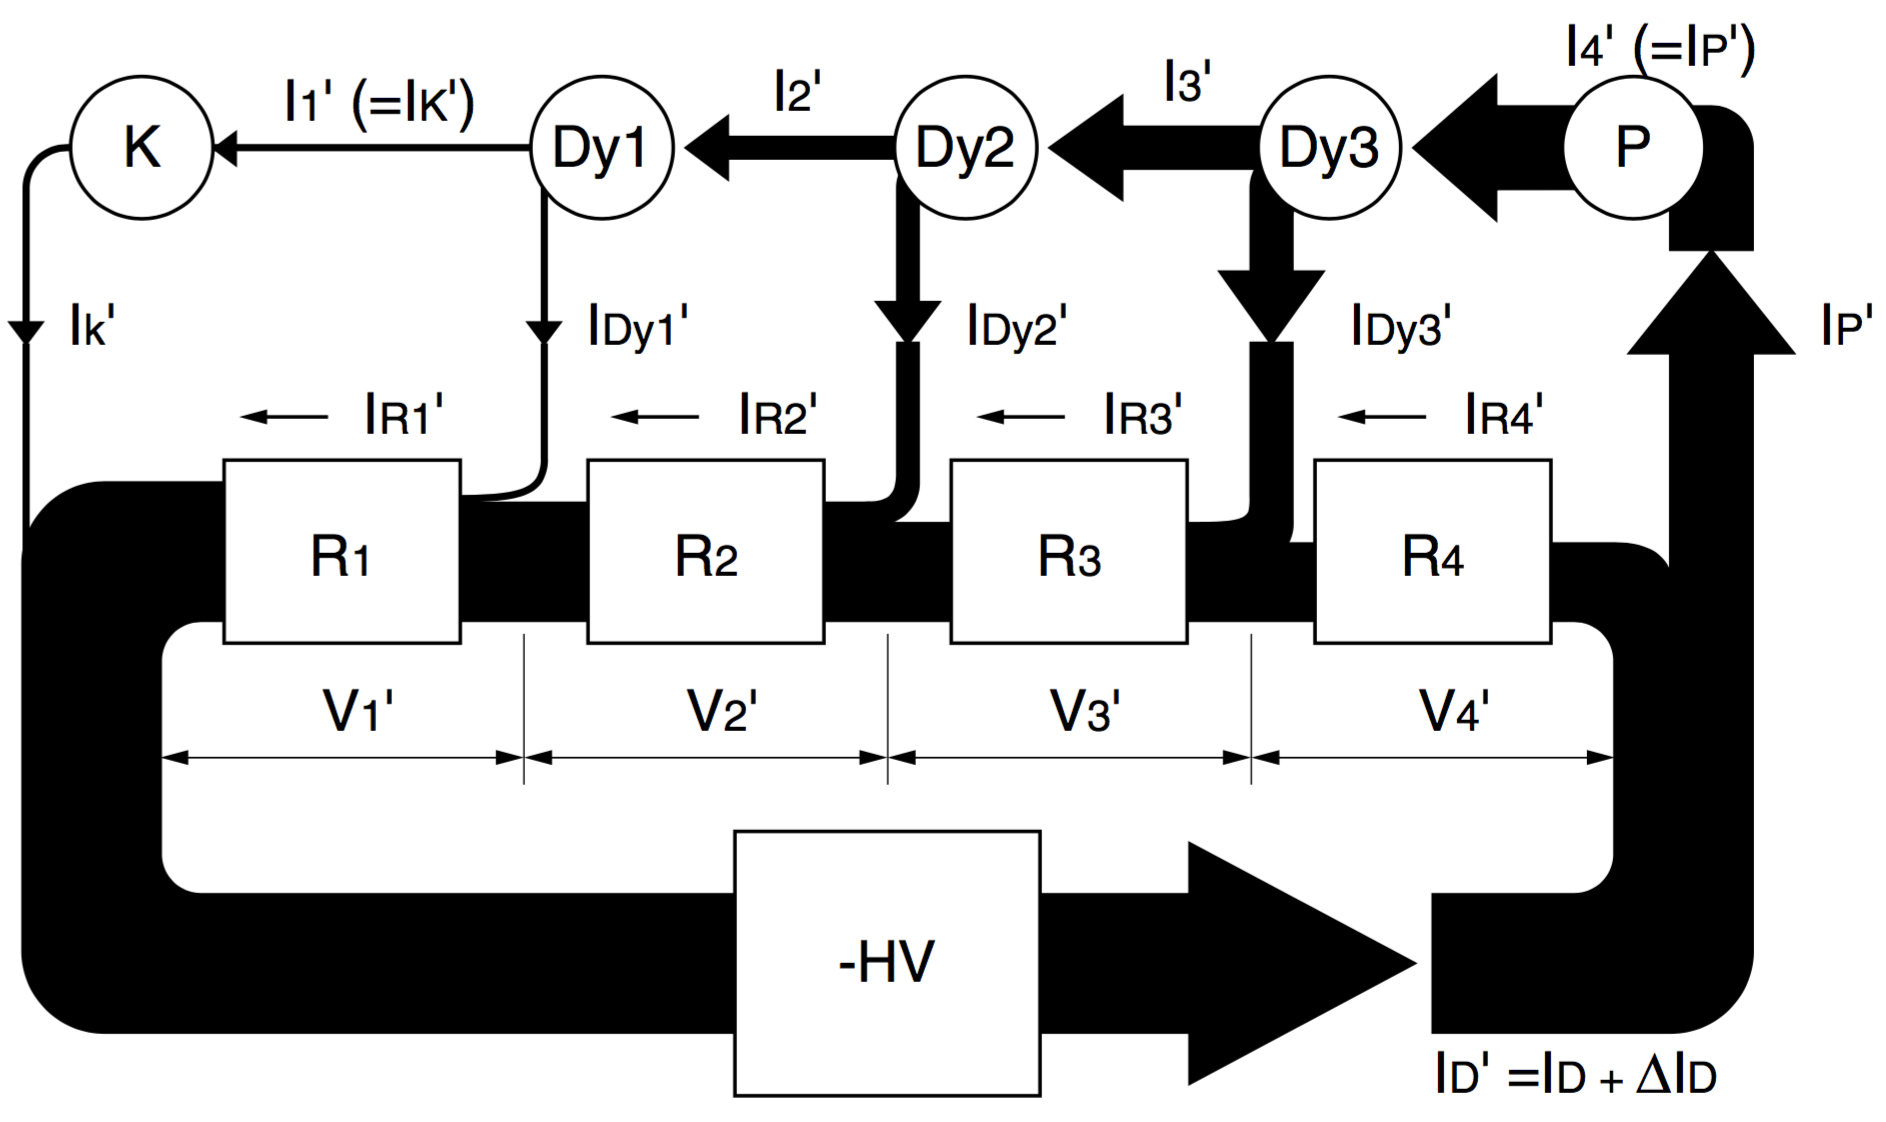
\includegraphics[width=0.9\textwidth]{chap/dynamic_range/fig/pmt_current_distribution_hamamatsu}
	\caption{Caption here}
	\label{fig:figure1}
\end{figure}

\subsection{分压器电路的设计}
\label{sec:dynamic_range:hv_divider}

\section{大动态范围读出方案的原理验证}
\label{sec:dynamic_range:verification}

\subsection{LED的测试}
\label{sec:dynamic_range:led}

\subsection{宇宙线的测试}
\label{sec:dynamic_range:cosmic_ray}

\subsection{中能轻核束流的测试}
\label{sec:dynamic_range:ion_beam}
